\documentclass[12pt]{article}
% REQUIRED input files: quiz-setup.tex TAs-and-sections.tex

\usepackage[symbol,perpage]{footmisc} %this is for dagger footnotes
\usepackage{xcolor}
\usepackage{hyperref}
\hypersetup{
    colorlinks=true,
    linkcolor=blue,
    filecolor=magenta,      
    urlcolor=blue,
}
\usepackage{pdfpages}

\input quiz-setup
\newcommand{\version}{} 
\newcommand{\xzero}{}
\newcommand{\xone}{}
\newcommand{\xtwo}{}
\newcommand{\xthree}{}
\newcommand{\xfour}{}
\newcommand{\xfive}{}
\newcommand{\vecb}[1]{\mathbf{#1}}

\newcommand{\ExamName}{Quiz \#0\version}
% \newcommand{\CourseName}{Math 34A} % This functionality moved to quiz-setup.tex
% \renewcommand{\Quarter}{Spring 2017}

%these are for dagger footnotes
\DefineFNsymbols*{daggorath}{{$\dagger$}{$\ddagger$}{$\dagger\dagger$}{$\ddagger\ddagger$}}
\setfnsymbol{daggorath}
\renewcommand{\thefootnote}{\fnsymbol{footnote}}
%\end dagger footnotes stuff




\begin{document}
%%
%% Version A:
\renewcommand{\version}{}
\renewcommand{\xzero}{0.0}
\renewcommand{\xone}{1.3}
\renewcommand{\xtwo}{2.9}
\renewcommand{\xthree}{4.1}
\renewcommand{\xfour}{5.3}
\renewcommand{\xfive}{6.5}
% 
\begin{minipage}{0.25\linewidth}
  \CourseName\ \Quarter \\
  \ExamName \\[1em]
  \textbf{No calculators}\\[2em]
\end{minipage}
\hfill
\begin{minipage}[t]{0.4\linewidth}
  
\begin{tikzpicture}[x=26mm,y=16mm]
    \draw[thick,black] (0,0) rectangle (3,1);
    \node[\faintcolor,right] at (0,0.2) {\large\textsf{PRINT NAME}};
  \end{tikzpicture}
\end{minipage}
\hfill
\begin{minipage}{0.25\linewidth}
  \vspace*{-3.25em}
  \ \hfill
  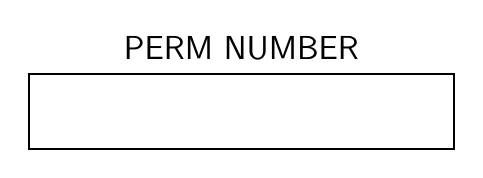
\begin{tikzpicture}[x=36mm,y=16mm]
    \node[\faintcolor] at (0.75,0.8) {\large\textsf{PERM NUMBER}};
    \draw[thick,black] (0,0) rectangle (1.5,0.6);
  \end{tikzpicture}
\end{minipage}
% \medskip
\vspace*{-0.25in}

%Put your answer in the 
%\begin{tikzpicture}[x=10mm,y=10mm,baseline=3mm] 
%  \draw[thick,black] (0,0) rectangle (3,1);
%  \node[\faintcolor] at (1.5,0.4) {\Huge\textsf{box}};
%\end{tikzpicture}
%provided.
\hfill
\begin{minipage}{0.5\linewidth}
%\begin{center}

  \textbf{TA:}\ 
  \parbox[t]{0.7in}{%
    \checkbox\ \TAOne \\
    \checkbox\ \TATwo 
  }
  %\parbox[t]{0.7in}{%
  %  \checkbox\ \TAThree\\
  %  \ \ \ 
  %}
  % \ 
  % \parbox[t]{4in}{%
  % \textbf{Section Time:}
  \hfill%\hspace*{0.25in}
  % \ 
  % \parbox[t]{4in}{%
  % \textbf{Section Time:}
  \textbf{Time:}
  \parbox[t]{0.55in}{%
    \checkbox\ 4:30 \\
    \checkbox\ 5:30
  }
  \quad
  \parbox[t]{0.55in}{%
    \checkbox\ 6:30 \\
    \checkbox\ 7:30 
  }
  % }
%  \textbf{TA:}\ 
%  \parbox[t]{0.95in}{%
%    \checkbox\ \TAOne
%  }
%  \parbox[t]{0.95in}{%
%    \checkbox\ \TATwo\\
%  }
%%  \parbox[t]{0.95in}{%
%%    \checkbox\ \TAThree
%%  }
%  \hspace*{0.5in} 
%  \parbox[t]{3in}{%
%    \textbf{Section Time:}
%    \parbox[t]{0.75in}{%
%      \checkbox\ 4:30 \\
%      \checkbox\ 5:30
%    }
%    \parbox[t]{0.75in}{%
%      \checkbox\ 6:30 \\
%      \checkbox\ 7:30
%    }
%  }
\end{center}
     % Uncomment this line to include the section where students
														   % mark which TA and section they are in. This is useful for
														   % in-person quizzes to make sure you've collected them all.
\end{minipage}
\noindent\hspace*{-2em}\rule{\textwidth+4em}{1pt}%

\mbox{}

In Math 34A this quarter we'll be using the ``Fixed Length" format for gradescope. This means that gradescope will expect the pages you submit to match the assignment pdf's pages. We have made the pdfs fillable, so that you can simply type your work and answers on the pdf and upload that. If you have a tablet such as an iPad, you can alternatively use your favorite app to write on the pdf with your stylus. 

\mbox{}

\begin{enumerate}
  \setcounter{problemnumber}{0}
\Problem $2+2=$ \answerbox{2}

\end{enumerate}

\bigskip



Sometimes a problem may have a lot of text to state the question, and there's nothing for you to write on that page. In this case you will find space for scratch work on the following page. You will need to show your work on exams. You do not need to do the following question today, it is presented here as an example. 
\bigskip
\begin{enumerate}
  \setcounter{problemnumber}{1}
\Problem Today we're making hot sauce. A Google search revealed a recipe that
calls for:
\begin{itemize}
\item 18 jalape\~nos.
\item 1 cup of water.
\item 2 cups of vinegar.
\end{itemize}
as well as some aromatics.
Spiciness of a pepper is measured in Scoville units, and jalape\~nos have 5000 Scoville units
each.
We only have 4 jalape\~nos on hand, but we have plenty of the following peppers: 

\begin{itemize}
\item Anaheim peppers (1000 Scoville units).
\item Serrano peppers (15,000 Scoville units).
\item Cayenne peppers (50,000 Scoville units).
\item Thai peppers (70,000 Scoville units).
\item Habanero peppers (150,000 Scoville units).
\item Ghost peppers (1,000,000 Scoville units)
\item Carolina reapers (2,000,000 Scoville units)
\end{itemize}

\begin{enumerate}[label=]\item
\begin{enumerate}[label=\roman*)]

\item What is the hottest pepper we could include without our hot sauce becoming spicier
than the original recipe?
\item You decide to use all four of your jalape\~nos, and use serrano peppers to complete
the recipe. How many serranos should you use if you want to make a hot sauce that
is exactly as spicy as the original recipe?
\item You're really curious about the flavor of the Carolina reaper, but you want to dilute
the spiciness with water/vinegar. How many cups of water do you need to add to a Carolina reaper to make hot
sauce that is as spicy as the original recipe?
\end{enumerate}
\end{enumerate}


\pagebreak

  \setcounter{problemnumber}{1}
\Problem Scratch work:

\vfill

Answers: (You can just write ``42" in all boxes)
\begin{enumerate}[label=(\roman*)]
\item \answerbox{3}
\item \answerbox{3}
\item \answerbox{3}
\end{enumerate}

\bigskip

\Problem Now it's time to export your pdf and upload to gradescope. Here is how to do this with  fillable pdf:

\bigskip
\includepdf[pages=-,pagecommand={},width=\textwidth]{examinstructions.pdf}


For those of you with a tablet, make sure you know how to export a PDF from your favorite note-taking app. Sometimes students take a screenshot of their iPad and submit that, but it's a really clunky way to do things. Here are some resources: 
\begin{itemize}
\item\href{https://support.goodnotes.com/hc/en-us/articles/360000630495-Exporting-documents-or-pages-in-GoodNotes-5}{\underline{Exporting documents or pages in GoodNotes 5}} 
\item \href{https://support.gingerlabs.com/hc/en-us/articles/205228298-Exporting-Notes}{\underline{Exporting Notes in Notability}}
\end{itemize}
 In either case, the process mostly amounts to ``look for the Share \includegraphics[scale=.15]{ios14-notes-share-icon} button". 

\bigskip
That's it! This is going to be a great quarter. Now test what you've learned by uploading this quiz to gradescope. 


\end{enumerate}

\end{document}
